\documentclass[tikz]{standalone}

% tikz
\usepackage{tikz, pgfplots}
% i wish external worked but idk it sucks
%\usetikzlibrary{external}
%\tikzexternalize[prefix=figures/]

% for function graph
\usetikzlibrary{positioning}
\usetikzlibrary{shapes.geometric}
\usetikzlibrary{positioning}
\tikzset{
dot/.style = {circle, fill=#1, minimum size=5pt,
              inner sep=0pt, outer sep=0pt},
dot/.default = black % size of the circle diameter
}

 % for braces
\usetikzlibrary{decorations.pathreplacing}
% for hashing area
\usetikzlibrary{patterns}
% tableaux var, signe
% source https://www.sqlpac.com/fr/documents/latex-package-tkz-tab-tikz-tableaux-de-signes-et-de-variations-de-fonctions.html
\usepackage{tkz-tab}
\input{../colors}
% Schwartz
\renewcommand{\S}{\mathcal{S}} % \S est le signe paragraphe normalement

% corps
\newcommand{\C}{\mathcal{C}}
\newcommand{\R}{\mathbb{R}}
\newcommand{\Rnn}{\mathbb{R}^{2n}}
\newcommand{\Z}{\mathbb{Z}}
\newcommand{\N}{\mathbb{N}}
\newcommand{\Q}{\mathbb{Q}}

% domain
\newcommand{\D}{\mathcal{D}}

% order notations
\renewcommand{\O}{\mathcal{O}}

% japanese bracket
\newcommand{\japb}[1]{\langle #1 \rangle}

% arrows over partial derivatives
\newcommand{\lp}{\overleftarrow{\partial}}
\newcommand{\rp}{\overrightarrow{\partial}}

% quantization
\newcommand{\h}{\hbar}
\newcommand{\Opht}{\textrm{Op}_{\h}^{t}}
\newcommand{\Op}[2][\hbar]{\textrm{Op}_{#1}^{#2}}

% omega functions
\newcommand{\omegap}[2][\rho_0]{\omega(\partial_{#1},\partial_{#2})}
\newcommand{\omegar}[2][\rho_0]{\omega(#1,#2)}

\begin{document}
%
	% page 1
	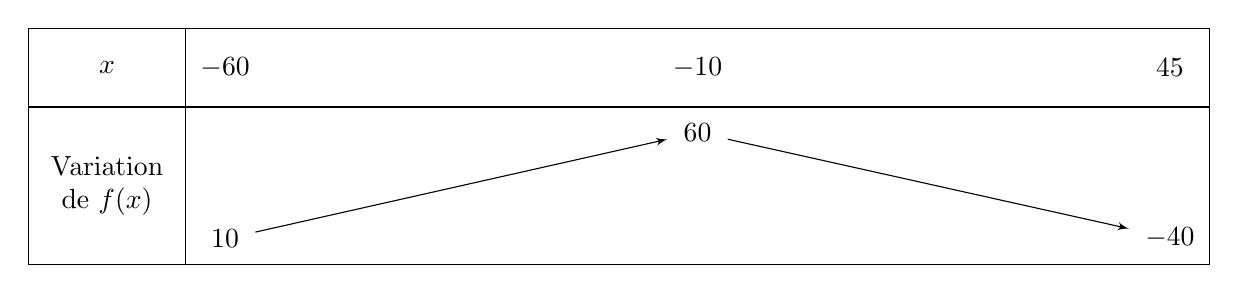
\begin{tikzpicture}
		\tkzTabInit
		 %[lgt=3,espcl=1.5]
	       		{$x$ / 1 , Variation de $f(x)$ / 2}
	       		{$-60$,, $-10$,, $45$}
	       		
		\tkzTabVar
			{-/$10$, R/, +/$60$, R/, -/$-40$}
	\end{tikzpicture}
	
	% page 2
	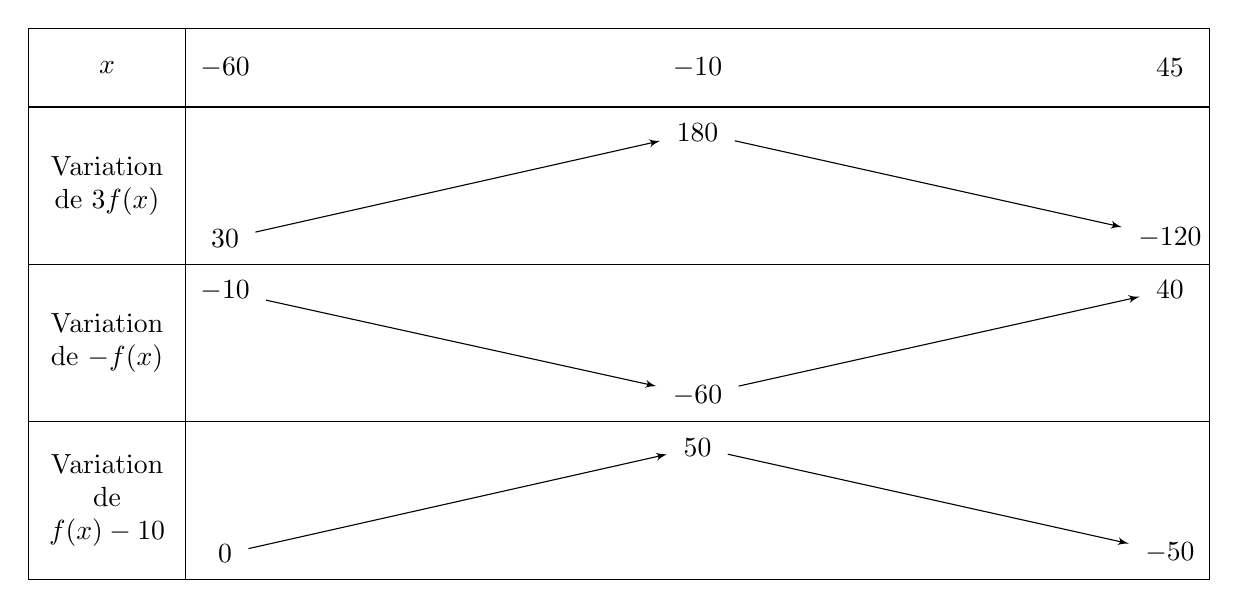
\begin{tikzpicture}
		\tkzTabInit
		 %[lgt=3,espcl=1.5]
	       		{$x$ / 1 , Variation de $3f(x)$ / 2, Variation de $-f(x)$ / 2, Variation de $f(x)-10$ / 2}
	       		{$-60$,, $-10$,, $45$}
	       		
		\tkzTabVar
			{-/$30$, R/, +/$180$, R/, -/$-120$}
		\tkzTabVar
			{+/$-10$, R/, -/$-60$, R/, +/$40$}
		\tkzTabVar
			{-/$0$, R/, +/$50$, R/, -/$-50$}
	\end{tikzpicture}
%
\end{document}